Figure \ref{fig:stx:expressions} specifies the syntax of all CML \emph{expressions}.
It also lists them in their order of precedence.
Observe that the grammar in figure \ref{fig:stx:expressions} has left
recursions, and thus is ambiguous.
However, ANTLR \cite{antlr} will use the order in which the alternatives
are listed in order to resolve the ambiguity,
and so define the precedence among the operators.
Also, according to ANTLR,
and as required by CML,
all expressions in the grammar are left-to-right associative,
except for the \emph{exponentiation expression},
which is right-to-left associative,
as defined by the \textbf{<assoc=right>} clause.

\begin{figure}
\verbatimfont{\small}
\lstinputlisting[language=antlr]{grammar/Expressions.txt}
\caption{Expressions Syntax}
\label{fig:stx:expressions}
\end{figure}

Figure \ref{fig:meta:expression} presents the \emph{Expression} metamodel
in an EMOF \cite{mof} class diagram.
For each kind of \emph{expression} parsed by the compiler,
an instance of an \emph{Expression} subclass will be created,
and its properties will be assigned
according to parsed information:

\begin{itemize}

\item \emph{kind}:
a \emph{String} value matching the \emph{Expression} subclass;
for example, for the \emph{Literal} subclass, \textbf{kind = "literal"}.

\item \emph{type}:
a derived attribute that computes the \emph{Type} of the \emph{expression};
each \emph{Expression} subclass will do its own \emph{Type} computation
by providing its own definition for this derived attribute.

\end{itemize}

\begin{figure}
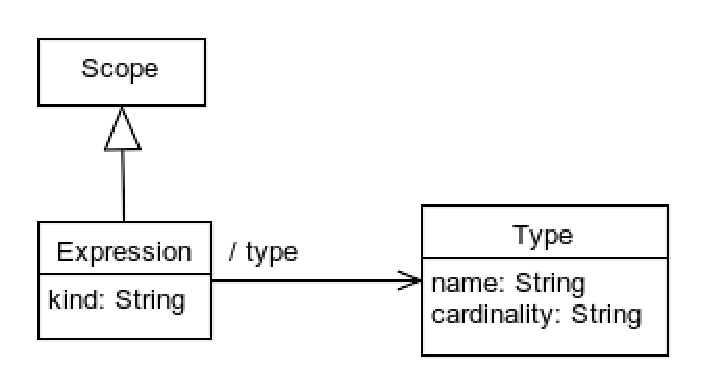
\includegraphics[width=\textwidth]{metamodel/expression}
\caption{Expression Metamodel}
\label{fig:meta:expression}
\end{figure}
